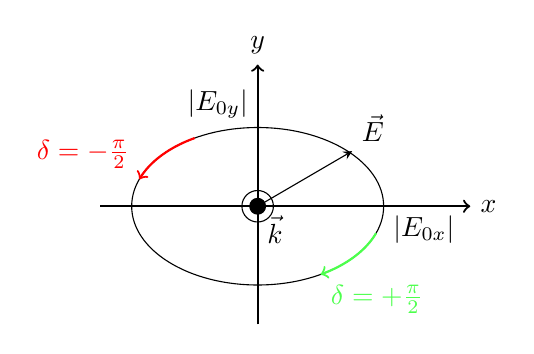
\begin{tikzpicture}
	% Achsen zeichnen
	\draw[->,thick] (-2,0) -- (2.7,0) node[right] {$x$};
	\draw[->,thick] (0,-1.5) -- (0,1.8) node[above] {$y$};
	%Plot
	%\draw[style=dashed] (-1.27,-1.05) rectangle (1.27,1.05);
	\draw (0, 0) ellipse (1.6 and 1);
	\draw(1.6,0) node[below right] {$|E_{0x}|$} ;
	\draw(0,1.3) node[left] {$|E_{0y}|$} ;
	\draw[->,>=stealth] (0,0)--(1.2,0.7) node[above right] {$\vec{E}$};
	%\draw[->,color=green] (40:1) arc (40:160:1.3);
	\draw [->,thick,color=green!70] plot[domain=340:300] ({cos(\x)*1.6},{sin(\x)}) node[below right] {$\delta = +\frac{\pi}{2}$};
	\draw [->,thick,color=red] plot[domain=120:160] ({cos(\x)*1.6},{sin(\x)}) node[above left] {$\delta = -\frac{\pi}{2}$};
	\draw (0, 0) circle (.2);
	\draw[fill=black] (0, 0) circle (.1);
	\draw (0,0) node[below right] {$\vec{k}$};
\end{tikzpicture}